\section{Perché Angular?}
Date queste premesse l'elaborato si pone come obbiettivo quello di mostrare le funzionalità di ottimizzazione delle performance che il framework angular offre agli sviluppatori.
\newline
Nato nel 2016 come evoluzione di angularjs e mantenuta da un team indipendente di sviluppatori google, la libreria viene ormai adottata sia per lo sviluppo di single page application ad alte prestazioni sia per la costruzione di frontend web.
\newline
La libreria offre molte possibilità agli sviluppatori
\begin{itemize}
    \item La possibilita di fare testing realtime dell'applicazione
    \item Alte prestazioni offerte dal meccanismo di change detection
    \item Alta flessibilità e scalabilità delle applicazioni
\end{itemize}
La libreria viene inoltre utilizzata da molte grandi realtà quali IBM Samsung e Paypal
\newline
\begin{figure}[H]
   \centering
   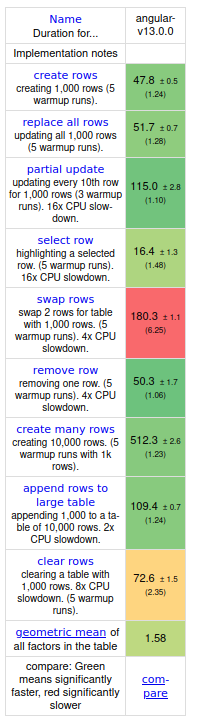
\includegraphics[scale=0.4]{resources/angular-performance.png}
\caption{test prestazioni libreria angular}
\end{figure}
